\documentclass{standalone}
\usepackage{hsbcommon}
\begin{document}
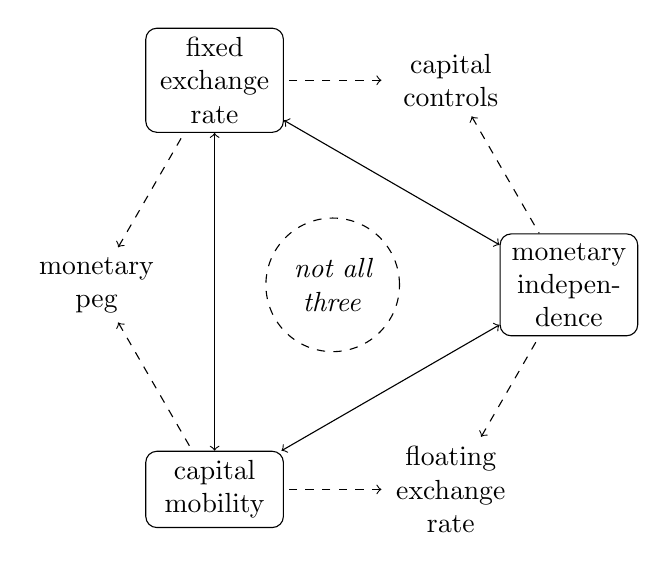
\begin{tikzpicture}
    \tikzset{
        policy/.style={
            text width=10ex,
            align=center,
            draw,
            rounded corners
        },
        result/.style={
            text width=10ex,
            align=center
        }
    }
    \foreach [count=\i] \mypolicy/\myresult in {
        fixed exchange rate     /   floating exchange rate,
        capital mobility        /   capital controls,
        monetary independence   /   monetary peg%        
    }
    {
        \node[policy] (P\i) at (\i*120:3) {\mypolicy};
        \node[result] (R\i) at (180+\i*120:3) {\myresult};
    }
    \foreach \i in {1,2,3}{
      \foreach \ii in {1,2,3}{
        \ifnum\i<\ii
          \draw[<->] (P\i) -- (P\ii);
        \fi
        \ifnum\i=\ii\else \draw[<-,dashed] (R\i) -- (P\ii); \fi
      }
    }
    \node[text width=8ex,align=center,circle,draw,dashed] at (0:0) {\textit{not all three}};
            
\end{tikzpicture}
\end{document}